\newcommand{\object}[3]{
\fbox{
\begin{tabular}[h!]{| p{7cm} |}
	\hline
	\textbf{#1} \\ \hline\hline
	\begin{mylist} #2 \end{mylist} \\ \hline
	\begin{mylist} #3 \end{mylist} \\ \hline

\end{tabular}
}
}

\newenvironment{mylist}{
	\begin{enumerate}[label=+]
}{
	\end{enumerate}
}

\section{Object Models}

\begin{figure}[h!]
\begin{center}
	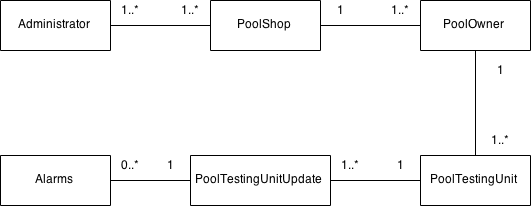
\includegraphics[width=15cm]{images/ObjectRelations}
	\caption{relationships between the main classes in the system}
\end{center}
\end{figure}

\par
There can be multiple administrators in the SPACS system that manage all the PoolShops. Each PoolOwner can only be registered at one PoolShop, and each PoolTestingUnit can only be linked to one PoolOwner. The Administrator, PoolShop and PoolOwner objects all contain information about a single person.

\subsection{Objects}
\subsubsection{User}
User is the class that all users of the system will fall under. It ensures a minimum amount of information is collected about each user and will implement all the basic instructions needed for interacting with the objects.

\object{User}
{
	\item id
	\item title
	\item name
	\item address 
	\item email\_address
	\item phone\_number
	\item mobile\_number
}
{
	\item
}

\subsubsection{Administrator, PoolShop and PoolOwner}
These are all extensions of the User object and will implement any extra methods that they do not inherit. Due to the way python works, these objects should have no methods.

\object{Administrator(User)}
{
	\item 
}
{
	\item
}

\object{PoolShop(User)}
{
	\item pool\_owners
}
{
	\item 
}

\object{PoolOwner(User)}
{
	\item pool\_testing\_units
}
{
	\item
}

\subsubsection{PoolTestingUnit}
Pool Testing Units are mostly passive users of the system and have the sole role of providing information to the system. They are closely linked to their PoolOwner. Again, due to the way python works this object should have no methods.

\object{PoolTestingUnit}
{
	\item pool\_id
	\item length
	\item width
	\item depth
	\item volume
	\item above\_ground
	\item material
						
}
{
	\item
}